\documentclass[tikz, border=10pt]{standalone}
\usepackage{tikz}
\usetikzlibrary{shapes.geometric, arrows.meta, positioning, fit, backgrounds}
\usepackage{xcolor}

% Definición de tus colores
\definecolor{primarygreen}{HTML}{2E7D32}
\definecolor{softgreen}{HTML}{E8F5E9}
\definecolor{primaryblue}{HTML}{1976D2}
\definecolor{softblue}{HTML}{E3F2FD}
\definecolor{accentorange}{HTML}{E65100}
\definecolor{darkgray}{HTML}{333333}
\definecolor{lightgray}{HTML}{F5F5F5}


\begin{document}

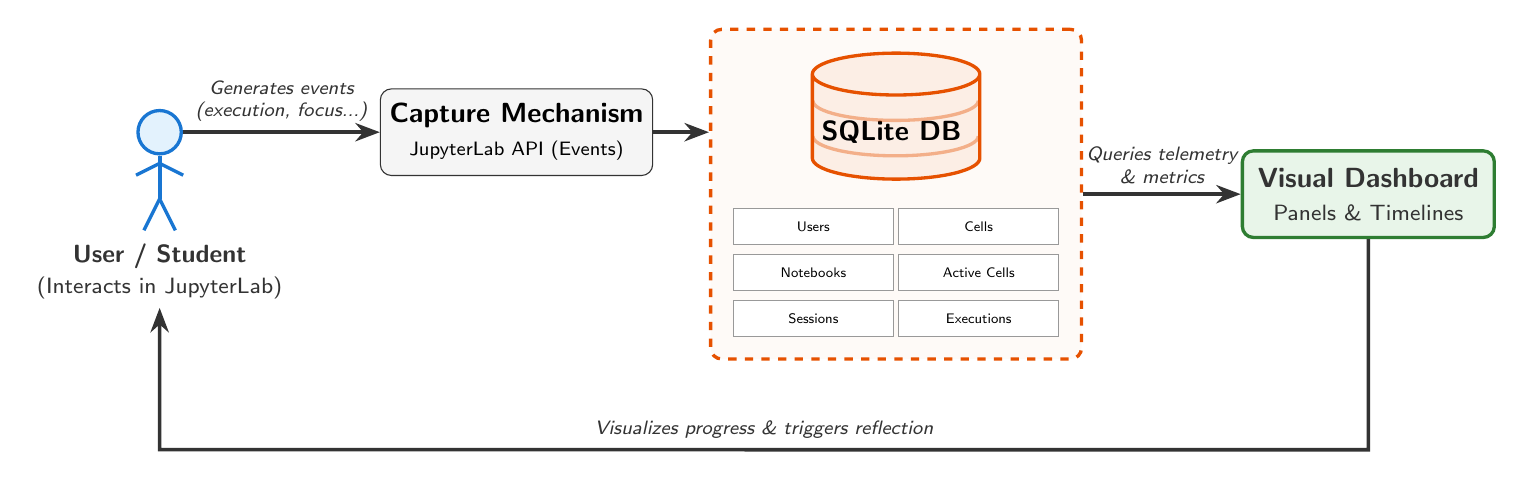
\begin{tikzpicture}[
    font=\sffamily,
    >=Stealth,
    % Estilos de bloques
    dashblock/.style={
        rectangle, 
        draw=primarygreen, 
        fill=softgreen, 
        rounded corners, 
        minimum width=3.2cm, 
        minimum height=1.1cm, 
        align=center, 
        line width=1.2pt,
        text=darkgray
    },
    tableblock/.style={
        rectangle, 
        draw=darkgray!50, 
        fill=white, 
        minimum width=1.8cm, 
        minimum height=0.45cm, 
        align=center, 
        text width=1.8cm,
        font=\sffamily\tiny
    },
    dbshape/.style={
        cylinder, 
        draw=accentorange, 
        fill=accentorange!10, 
        shape border rotate=90, 
        aspect=0.25, 
        minimum width=1.4cm, 
        minimum height=1.6cm, 
        line width=1.2pt, 
        align=center
    },
    flow/.style={
        draw=darkgray, 
        ->, 
        line width=1.3pt
    },
    flowtext/.style={
        font=\sffamily\scriptsize\itshape, 
        align=center, 
        text=darkgray
    }
]

    % ==========================================
    % 1. USER REPRESENTATION (Izquierda)
    % ==========================================
    \begin{scope}[local bounding box=userbox]
        % Cabeza
        \node[circle, draw=primaryblue, fill=softblue, minimum size=0.55cm, line width=1.2pt] (head) at (0,0) {};
        % Torso
        \draw[primaryblue, line width=1.5pt] (head.south) -- ++(0,-0.55) coordinate (torso);
        % Brazos
        \draw[primaryblue, line width=1.2pt] (head.south)++(0,-0.1) -- ++(-0.3,-0.15);
        \draw[primaryblue, line width=1.2pt] (head.south)++(0,-0.1) -- ++(0.3,-0.15);
        % Piernas
        \draw[primaryblue, line width=1.2pt] (torso) -- ++(-0.2,-0.4);
        \draw[primaryblue, line width=1.2pt] (torso) -- ++(0.2,-0.4);
        % Etiqueta
        \node[below=0.45cm of torso, font=\sffamily\bfseries\small, text=darkgray, align=center] {User / Student\\ \mdseries\footnotesize(Interacts in JupyterLab)};
    \end{scope}

    % ==========================================
    % 2. CAPTURE MECHANISM (Centro-Izquierda)
    % ==========================================
    \node[rectangle, draw=darkgray, fill=lightgray, rounded corners, right=2.5cm of head, yshift=0cm, minimum width=3.0cm, minimum height=1.1cm, align=center] (api) {
        \textbf{Capture Mechanism} \\ 
        \scriptsize{JupyterLab API (Events)}
    };

    % ==========================================
    % 3. DATABASE STRUCTURE (Centro-Derecha, 2 columnas)
    % ==========================================
    \node[dbshape, right=2.0cm of api] (sqlite) {
        \textbf{SQLite DB}
    };

    % Líneas 3D del cilindro
    \draw[accentorange, opacity=0.4, line width=1.2pt] 
        ([yshift=0.4cm, xshift=0.8pt]sqlite.west) arc (180:360:1.05cm and 0.25cm);
    \draw[accentorange, opacity=0.4, line width=1.2pt] 
        ([yshift=-0.05cm, xshift=0.8pt]sqlite.west) arc (180:360:1.05cm and 0.25cm);

    % Tablas en 2 columnas
    \node[tableblock, below=0.35cm of sqlite, xshift=-1.05cm] (t1) {Users};
    \node[tableblock, below=0.12cm of t1] (t2) {Notebooks};
    \node[tableblock, below=0.12cm of t2] (t3) {Sessions};

    \node[tableblock, below=0.35cm of sqlite, xshift=1.05cm] (t4) {Cells};
    \node[tableblock, below=0.12cm of t4] (t5) {Active Cells};
    \node[tableblock, below=0.12cm of t5] (t6) {Executions};

    % Contenedor DB
    \begin{scope}[on background layer]
        \node[draw=accentorange, dashed, line width=1.2pt, fill=accentorange!3, rounded corners, inner sep=8pt, fit=(sqlite) (t1) (t3) (t4) (t6)] (dbcontainer) {};
    \end{scope}

    % ==========================================
    % 4. VISUAL DASHBOARD (Derecha total)
    % ==========================================
    \node[dashblock, right=2.0cm of dbcontainer.east, anchor=west] (dash) {
        \textbf{Visual Dashboard} \\ 
        \footnotesize{Panels \& Timelines}
    };

    % ==========================================
    % FLUJOS Y CONEXIONES (Lineal de Izq a Der + Retorno Inferior)
    % ==========================================
    
    % Usuario -> Captura
    \path[flow] (head.east) -- node[flowtext, above] {Generates events\\(execution, focus...)} (api.west);
    
    % Captura -> Base de Datos
    \path[flow] (api.east) -- (dbcontainer.west |- api.east);
    
    % Base de Datos -> Dashboard
    \path[flow] (dbcontainer.east |- dash.west) -- node[flowtext, above] {Queries telemetry\\\& metrics} (dash.west);
    
    % Feedback: Dashboard -> Usuario (Por debajo de todo el diagrama)
    \draw[flow] (dash.south) -- ++(0,-2.675cm) 
        -- node[flowtext, above, pos=0.5] {Visualizes progress \& triggers reflection} 
        ([yshift=-1.8cm]userbox.south) -- (userbox.south);

\end{tikzpicture}

\end{document}